\chapter{Conception du Laboratoire Réseau}

\section{Introduction}

Avant de développer le système \textbf{Automated Network Self-Defense System (ANSDS)}, il a été indispensable de concevoir une plateforme de test permettant de reproduire un environnement réseau réaliste et entièrement maîtrisé. Ce laboratoire constitue la base expérimentale du projet et permet de développer, de tester et de valider chaque composant du système dans des conditions proches d'une infrastructure d'entreprise.

L'environnement a été réalisé à l'aide de GNS3 \cite{gns3_docs} en intégrant un routeur Cisco IOS \cite{cisco_ios}, un commutateur Ethernet, un serveur Ubuntu, une machine Kali Linux ainsi qu'un accès Internet via un mécanisme de traduction d'adresses réseau (Network Address Translation -- NAT). Cette architecture offre un environnement adapté à l'étude du protocole SSH \cite{rfc4253}, à la capture des paquets réseau ainsi qu'au développement des mécanismes de détection et de réponse automatique.

Avant de commencer les phases de détection d'attaques, l'ensemble des équipements a été configuré puis validé afin de garantir le bon fonctionnement des communications réseau.

\section{Objectifs du laboratoire}

La mise en place du laboratoire poursuit plusieurs objectifs techniques indispensables au développement du projet ANSDS :

\begin{itemize}
    \item Concevoir une infrastructure réseau représentative d'un environnement réel.
    \item Déployer un serveur Ubuntu jouant le rôle de machine victime.
    \item Déployer une machine Kali Linux représentant l'attaquant.
    \item Configurer le routage et l'accès Internet à l'aide d'un routeur Cisco.
    \item Mettre en œuvre la traduction d'adresses (NAT).
    \item Valider l'ensemble des communications réseau avant le développement des mécanismes de sécurité.
    \item Préparer un environnement permettant l'analyse du trafic SSH avec Wireshark.
    \item Fournir une plateforme stable pour les futures phases de détection et de réponse automatique.
\end{itemize}

\section{Architecture générale du laboratoire}

L'architecture du laboratoire a été développée sous GNS3 \cite{gns3_docs} afin de reproduire une infrastructure réseau simple, stable et facilement reproductible.

Elle est constituée des éléments suivants :

\begin{itemize}
    \item un routeur Cisco IOS assurant le routage des paquets et l'accès Internet ;
    \item un commutateur Cisco reliant les différentes machines du réseau local ;
    \item un serveur Ubuntu représentant la machine victime ;
    \item une machine Kali Linux représentant l'attaquant ;
    \item un nœud NAT permettant l'accès aux ressources Internet.
\end{itemize}

La Figure~\ref{fig:topology} présente l'architecture générale du laboratoire utilisée durant la totalité de la première phase du projet.

\begin{figure}[htbp]
    \centering
    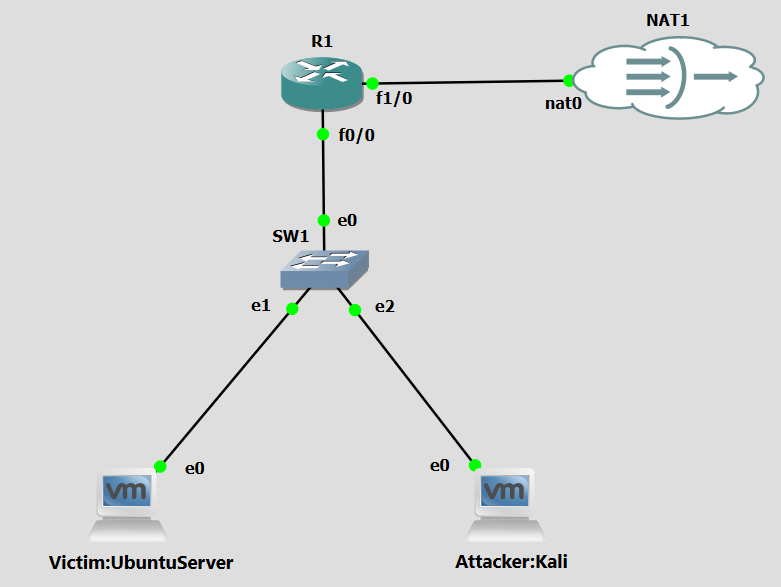
\includegraphics[width=\textwidth]{figures/01-network-topology.png}
    \caption{Architecture générale du laboratoire réseau développé sous GNS3}
    \label{fig:topology}
\end{figure}

Cette architecture permet d'isoler totalement l'environnement de test tout en offrant les fonctionnalités nécessaires au développement du système ANSDS. Elle constitue la base sur laquelle seront réalisées les captures réseau, les attaques SSH simulées ainsi que les mécanismes de détection et de défense présentés dans les chapitres suivants.

\section{Équipements du laboratoire}

L'infrastructure du laboratoire repose sur plusieurs équipements réseau ayant chacun une fonction bien définie. Ensemble, ils permettent de reproduire un environnement représentatif d'un réseau d'entreprise tout en offrant une plateforme adaptée au développement et à la validation du système ANSDS.

Les sous-sections suivantes présentent le rôle de chaque équipement ainsi que les principales configurations réalisées.

\subsection{Routeur Cisco}

Le routeur Cisco constitue l'élément central de l'architecture réseau. Il assure le routage des paquets entre le réseau local et Internet, ainsi que la mise en œuvre du mécanisme de traduction d'adresses (NAT). Il jouera également un rôle essentiel dans les phases suivantes du projet, puisqu'il sera chargé d'appliquer automatiquement des listes de contrôle d'accès (ACL) afin de bloquer les adresses IP identifiées comme malveillantes \cite{cisco_ios}.

Le routeur utilisé est basé sur la plateforme Cisco 7200 et dispose de plusieurs interfaces FastEthernet permettant d'interconnecter le réseau local au nœud NAT de GNS3.

La Figure~\ref{fig:router-hardware} présente la configuration matérielle retenue pour le routeur.

\begin{figure}[htbp]
    \centering
    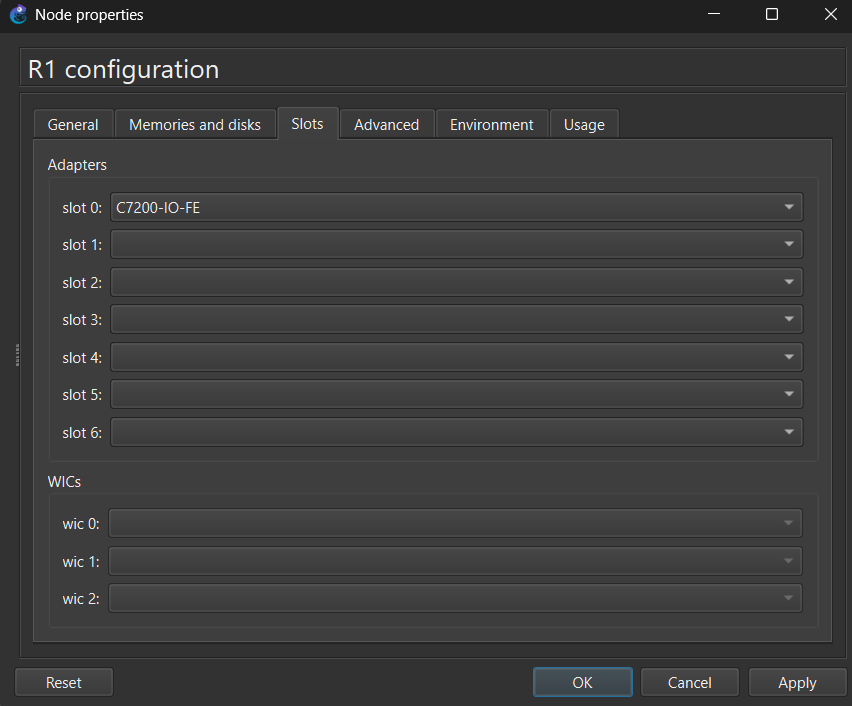
\includegraphics[width=0.85\textwidth]{figures/02-router-hardware.png}
    \caption{Configuration matérielle du routeur Cisco}
    \label{fig:router-hardware}
\end{figure}

La configuration IP des interfaces du routeur est présentée à la Figure~\ref{fig:router-ip}. L'interface FastEthernet0/0 est utilisée comme passerelle du réseau local tandis que l'interface FastEthernet1/0 assure la connexion vers Internet.

\begin{figure}[htbp]
    \centering
    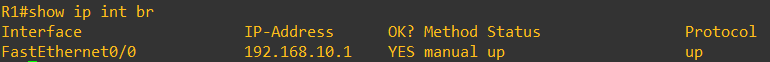
\includegraphics[width=0.70\textwidth]{figures/03-router-ip-configuration.png}
    \caption{Configuration IP des interfaces du routeur Cisco}
    \label{fig:router-ip}
\end{figure}

\subsection{Commutateur Cisco}

Le commutateur Cisco assure l'interconnexion des équipements du réseau local. Il relie le serveur Ubuntu, la machine Kali Linux et le routeur Cisco au sein du même segment Ethernet.

Aucune configuration spécifique n'a été nécessaire sur ce commutateur. Son rôle est exclusivement de fournir la connectivité de niveau 2 entre les différents équipements du laboratoire. Comme présenté à la Figure~\ref{fig:topology}, il constitue le point central des communications locales.

\subsection{Serveur Ubuntu}

Le serveur Ubuntu représente la machine victime du projet. Il héberge le service OpenSSH qui sera utilisé lors des différentes expérimentations de sécurité. Les futures attaques par force brute ainsi que les mécanismes de détection développés dans ANSDS cibleront cette machine.

Une configuration IP statique a été appliquée afin de garantir la stabilité de l'environnement de test. Le serveur utilise l'adresse IP 192.168.10.10/24 et la passerelle par défaut 192.168.10.1.

La configuration réseau du serveur est illustrée à la Figure~\ref{fig:ubuntu-network}.

\begin{figure}[htbp]
    \centering
    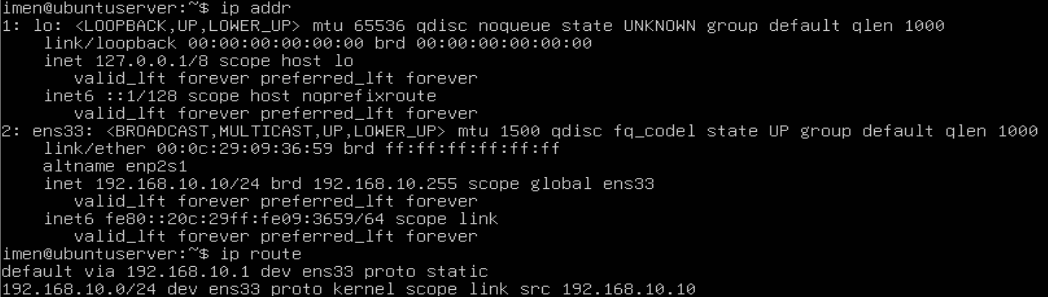
\includegraphics[width=0.90\textwidth]{figures/04-victim-network-configuration.png}
    \caption{Configuration réseau du serveur Ubuntu}
    \label{fig:ubuntu-network}
\end{figure}

\subsection{Machine Kali Linux}

La machine Kali Linux représente l'attaquant dans le laboratoire. Elle est utilisée pour établir les connexions SSH, générer les attaques simulées et valider le fonctionnement des mécanismes de détection et de réponse automatique.

Comme le serveur Ubuntu, cette machine possède une configuration IP statique afin d'assurer la reproductibilité des expérimentations. Son adresse IP est 192.168.10.20/24 et sa passerelle par défaut est 192.168.10.1.

La Figure~\ref{fig:kali-network} présente la configuration réseau de la machine Kali Linux.

\begin{figure}[htbp]
    \centering
    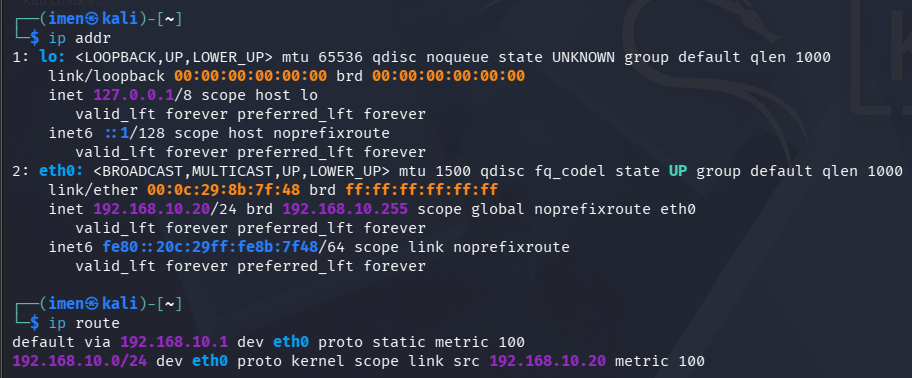
\includegraphics[width=0.90\textwidth]{figures/05-attacker-network-configuration.png}
    \caption{Configuration réseau de la machine Kali Linux}
    \label{fig:kali-network}
\end{figure}

\section{Plan d'adressage IP}

Afin d'assurer une communication stable entre les différents équipements du laboratoire, un plan d'adressage IP statique a été défini. Chaque équipement possède une adresse IP fixe facilitant les phases de développement, de test et de validation.

Le Tableau~\ref{tab:ip-addressing} présente le plan d'adressage adopté.

\begin{table}[htbp]
\centering
\caption{Plan d'adressage IP du laboratoire}
\label{tab:ip-addressing}

\begin{tabular}{llll}
\toprule
Équipement & Interface & Adresse IP & Passerelle \\
\midrule
Routeur Cisco & FastEthernet0/0 & 192.168.10.1/24 & --- \\
Serveur Ubuntu & ens33 & 192.168.10.10/24 & 192.168.10.1 \\
Kali Linux & eth0 & 192.168.10.20/24 & 192.168.10.1 \\
\bottomrule
\end{tabular}

\end{table}

L'ensemble des machines du réseau local appartient au sous-réseau \texttt{192.168.10.0/24}. Le routeur Cisco joue le rôle de passerelle par défaut et assure l'acheminement des paquets vers le réseau externe via le mécanisme de traduction d'adresses (NAT).

\section{Configuration NAT}

Afin de permettre aux machines virtuelles du laboratoire d'accéder au réseau Internet, une traduction d'adresses réseau (\textit{Network Address Translation} -- NAT) a été configurée sur le routeur Cisco \cite{cisco_ios}.

Le mécanisme retenu est le \textit{Port Address Translation} (PAT), également appelé surcharge NAT (\textit{NAT Overload}). Cette technique permet à plusieurs machines du réseau privé de partager une seule adresse IP publique correspondant à l'interface connectée au réseau externe.

Dans cette configuration, l'interface FastEthernet0/0 est définie comme interface interne (\textit{inside}), tandis que l'interface FastEthernet1/0 est configurée comme interface externe (\textit{outside}).

La Figure~\ref{fig:nat-configuration} présente la configuration NAT appliquée sur le routeur Cisco.

\begin{figure}[htbp]
    \centering
    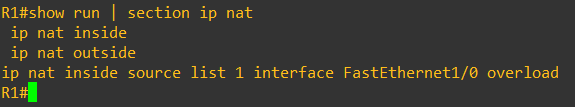
\includegraphics[width=0.95\textwidth]{figures/10-router-nat-configuration.png}
    \caption{Configuration NAT du routeur Cisco}
    \label{fig:nat-configuration}
\end{figure}

L'instruction \texttt{ip nat inside source list 1 interface FastEthernet1/0 overload} active le mécanisme PAT. Toutes les machines appartenant à la liste d'accès numéro 1 peuvent ainsi accéder au réseau externe en utilisant l'adresse IP de l'interface FastEthernet1/0.

Cette configuration constitue une étape essentielle du laboratoire, puisqu'elle garantit la connectivité Internet nécessaire à l'installation des paquets logiciels, aux mises à jour du système ainsi qu'aux différentes expérimentations réalisées durant le projet.

\section{Validation de l'environnement réseau}

Une fois la configuration des différents équipements terminée, plusieurs vérifications ont été réalisées afin de s'assurer du bon fonctionnement de l'environnement avant de débuter les expérimentations liées au système ANSDS.

Ces vérifications concernent notamment la version du système Cisco IOS ainsi que la connectivité Internet du laboratoire.

\subsection{Version Cisco IOS}

Le routeur utilisé dans le laboratoire exécute le système d'exploitation Cisco IOS. La vérification de la version installée permet de confirmer la compatibilité des fonctionnalités utilisées dans le cadre du projet, notamment le routage IP, la traduction d'adresses (NAT) et les listes de contrôle d'accès (ACL) \cite{cisco_ios}.

La Figure~\ref{fig:ios-version} présente les informations relatives à la version du système Cisco IOS.

\begin{figure}[htbp]
    \centering
    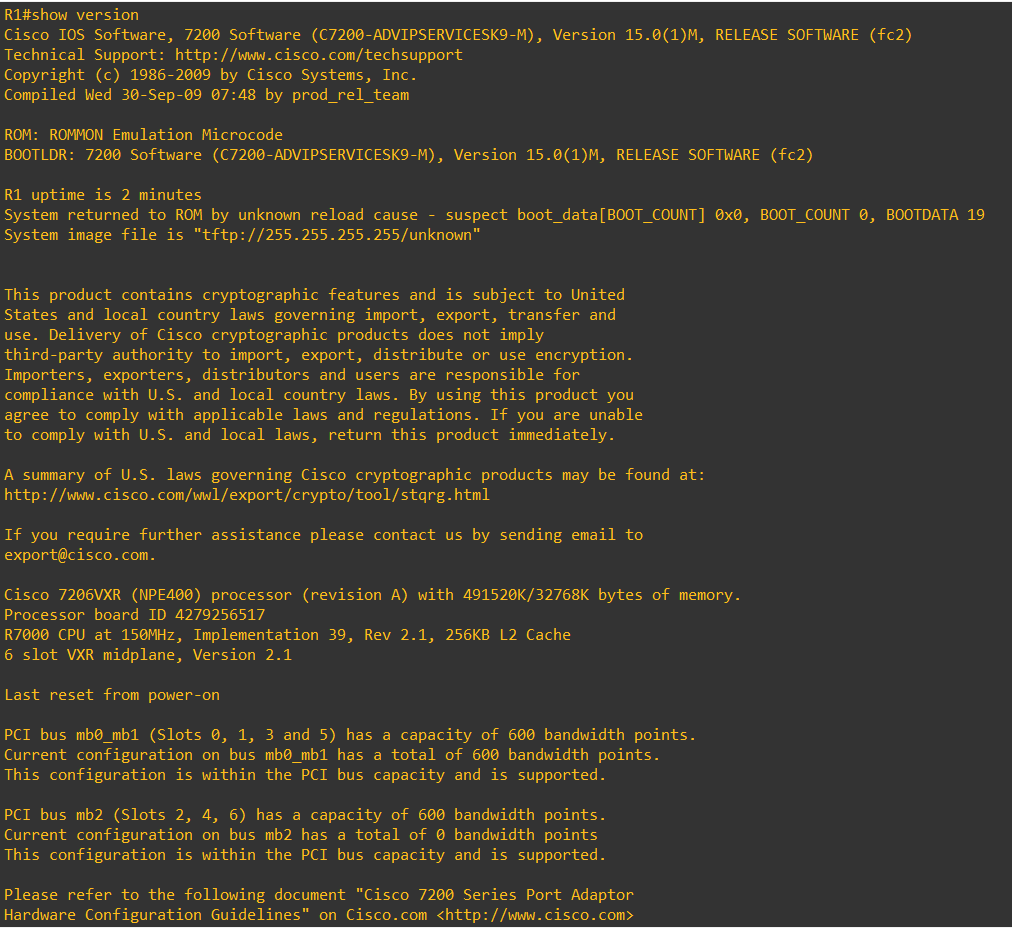
\includegraphics[width=0.95\textwidth]{figures/12-router-ios-version.png}
    \caption{Vérification de la version Cisco IOS}
    \label{fig:ios-version}
\end{figure}

\subsection{Validation de la connectivité Internet}

Après la configuration du mécanisme NAT, un test de connectivité a été réalisé afin de vérifier que le routeur était capable d'accéder au réseau Internet.

La réussite de ce test confirme le bon fonctionnement du routage ainsi que de la traduction d'adresses configurée précédemment.

La Figure~\ref{fig:internet-connectivity} présente le résultat de ce test.

\begin{figure}[htbp]
    \centering
    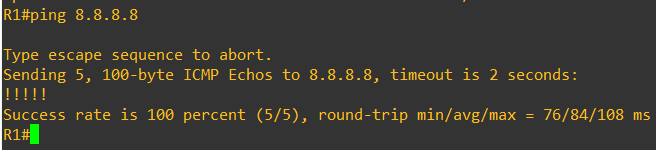
\includegraphics[width=0.90\textwidth]{figures/11-router-internet-connectivity.png}
    \caption{Validation de la connectivité Internet}
    \label{fig:internet-connectivity}
\end{figure}

La validation de ces deux éléments confirme que l'infrastructure réseau est correctement configurée et prête pour les phases de test et de développement du système ANSDS.

\section{Validation des communications réseau}

Une fois l'ensemble des équipements configurés, plusieurs tests de connectivité ont été réalisés afin de vérifier le bon fonctionnement de l'infrastructure réseau. Ces tests permettent de s'assurer que chaque machine peut communiquer correctement avec les autres équipements du laboratoire avant le déploiement des mécanismes de sécurité.

Les essais ont été réalisés à l'aide de la commande \texttt{ping}, qui permet de vérifier la disponibilité d'un équipement ainsi que la bonne configuration du routage.

\subsection{Communication entre le serveur Ubuntu et le routeur}

Le premier test consiste à vérifier que le serveur Ubuntu peut joindre la passerelle du réseau local.

La Figure~\ref{fig:ping-victim-router} montre que le routeur répond correctement aux requêtes ICMP envoyées par le serveur Ubuntu.

\begin{figure}[htbp]
    \centering
    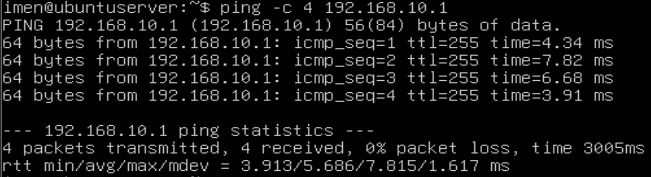
\includegraphics[width=0.90\textwidth]{figures/06-ping-victim-to-router.png}
    \caption{Test de connectivité entre le serveur Ubuntu et le routeur Cisco}
    \label{fig:ping-victim-router}
\end{figure}

\subsection{Communication entre Kali Linux et le routeur}

Le même test a été réalisé depuis la machine Kali Linux afin de vérifier sa connectivité avec la passerelle du réseau.

Comme illustré à la Figure~\ref{fig:ping-attacker-router}, les réponses ICMP confirment le bon fonctionnement de cette liaison.

\begin{figure}[htbp]
    \centering
    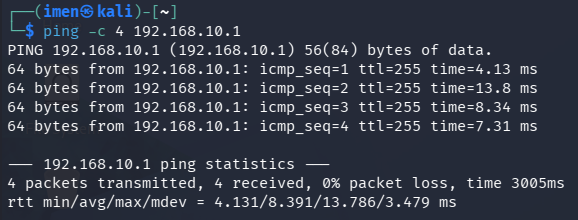
\includegraphics[width=0.90\textwidth]{figures/07-ping-attacker-to-router.png}
    \caption{Test de connectivité entre Kali Linux et le routeur Cisco}
    \label{fig:ping-attacker-router}
\end{figure}

\subsection{Communication entre le serveur Ubuntu et Kali Linux}

Une communication directe entre les deux machines virtuelles a ensuite été vérifiée.

La Figure~\ref{fig:ping-victim-attacker} montre que le serveur Ubuntu peut communiquer correctement avec la machine Kali Linux.

\begin{figure}[htbp]
    \centering
    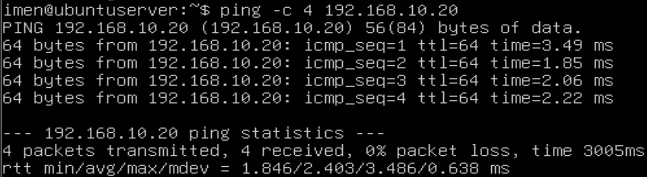
\includegraphics[width=0.90\textwidth]{figures/08-ping-victim-to-attacker.png}
    \caption{Communication entre le serveur Ubuntu et Kali Linux}
    \label{fig:ping-victim-attacker}
\end{figure}

\subsection{Communication entre Kali Linux et le serveur Ubuntu}

Enfin, le test inverse a été réalisé afin de confirmer la connectivité bidirectionnelle entre les deux machines.

Les résultats présentés à la Figure~\ref{fig:ping-attacker-victim} confirment que les échanges réseau sont fonctionnels dans les deux sens.

\begin{figure}[htbp]
    \centering
    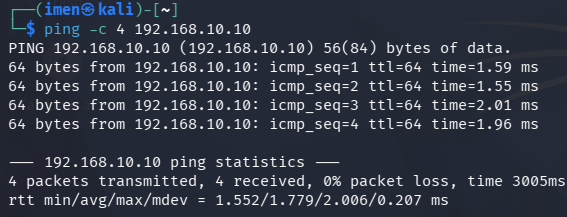
\includegraphics[width=0.90\textwidth]{figures/09-ping-attacker-to-victim.png}
    \caption{Communication entre Kali Linux et le serveur Ubuntu}
    \label{fig:ping-attacker-victim}
\end{figure}

Les différents tests de connectivité réalisés confirment le bon fonctionnement de l'infrastructure réseau. Le routage IP, les configurations des interfaces ainsi que les communications entre les différents équipements ont été validés avec succès. Cette étape garantit que le laboratoire est prêt pour l'installation et les tests du service SSH, qui constituent la base des expérimentations présentées dans la suite du projet.

\section{Validation du service SSH}

Le protocole Secure Shell (SSH) constitue l'élément central des expérimentations réalisées dans le cadre du projet ANSDS \cite{rfc4253}. Avant de développer les mécanismes de détection et de réponse automatique, il est indispensable de vérifier que le service SSH est correctement installé, actif et accessible depuis les autres équipements du laboratoire.

Plusieurs vérifications successives ont été réalisées afin de valider le bon fonctionnement du service.

\subsection{Installation du serveur OpenSSH}

Le serveur Ubuntu a été configuré afin d'héberger le service OpenSSH. Cette étape permet d'accepter les connexions SSH provenant de la machine Kali Linux.

La Figure~\ref{fig:ssh-installation} présente l'installation du serveur OpenSSH.

\begin{figure}[htbp]
    \centering
    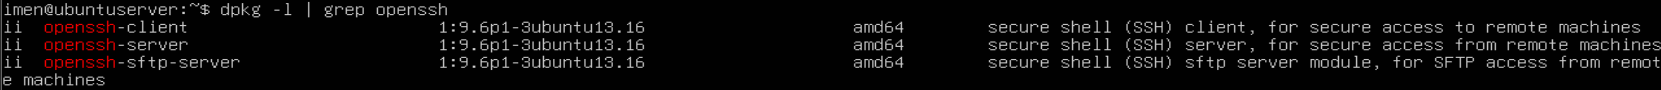
\includegraphics[width=0.95\textwidth]{figures/13-openssh-installation.png}
    \caption{Installation du serveur OpenSSH}
    \label{fig:ssh-installation}
\end{figure}

\subsection{Vérification de l'état du service}

Une fois l'installation terminée, le statut du service SSH a été vérifié afin de confirmer son bon fonctionnement.

Comme l'illustre la Figure~\ref{fig:ssh-status}, le service est correctement démarré et prêt à accepter les connexions entrantes.

\begin{figure}[htbp]
    \centering
    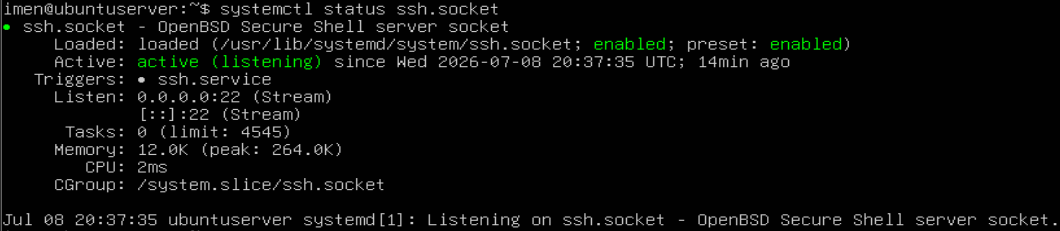
\includegraphics[width=0.95\textwidth]{figures/14-ssh-socket-status.png}
    \caption{Vérification de l'état du service SSH}
    \label{fig:ssh-status}
\end{figure}

\subsection{Vérification du port d'écoute}

Le fonctionnement du serveur SSH a également été validé en vérifiant que le port TCP 22 est en état d'écoute.

La Figure~\ref{fig:ssh-port} confirme que le service écoute correctement sur le port standard utilisé par le protocole SSH \cite{rfc4253}.

\begin{figure}[htbp]
    \centering
    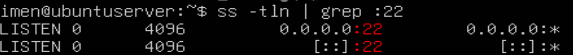
\includegraphics[width=0.90\textwidth]{figures/15-ssh-port-listening.png}
    \caption{Vérification de l'écoute du port TCP 22}
    \label{fig:ssh-port}
\end{figure}

\subsection{Validation d'une connexion SSH}

La dernière étape consiste à établir une connexion SSH entre la machine Kali Linux et le serveur Ubuntu.

La réussite de cette connexion confirme que l'ensemble des configurations réseau et du service SSH sont opérationnelles. Cette validation est essentielle, car toutes les expérimentations des chapitres suivants reposeront sur cette communication.

La Figure~\ref{fig:ssh-success} présente une connexion SSH réussie entre les deux machines.

\begin{figure}[htbp]
    \centering
    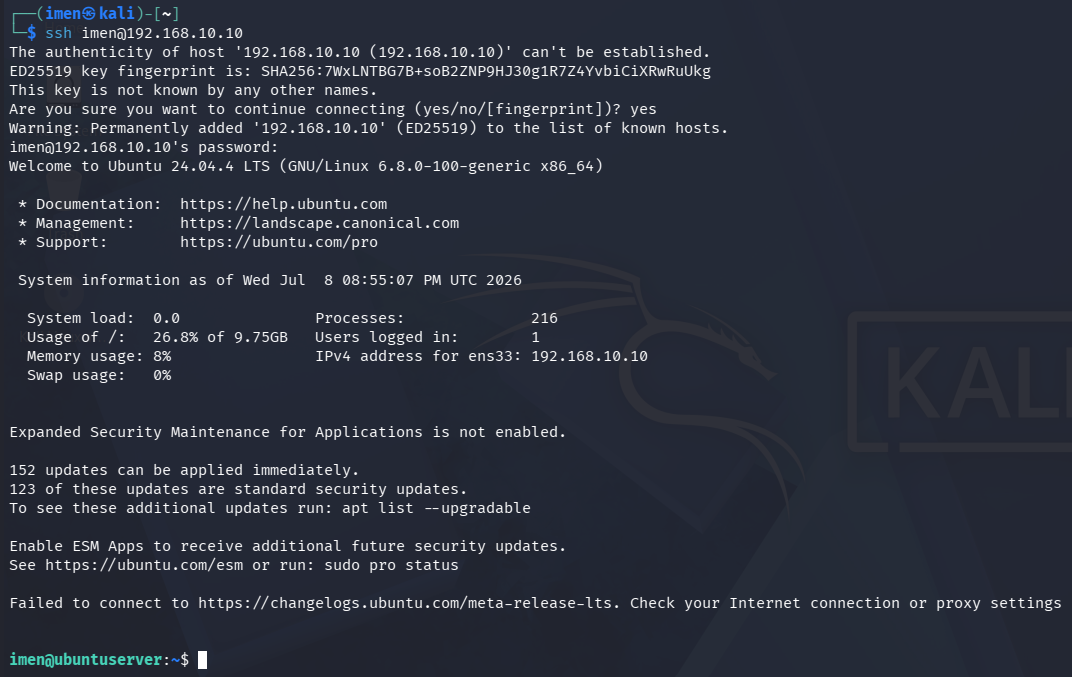
\includegraphics[width=0.95\textwidth]{figures/16-successful-ssh-connection.png}
    \caption{Connexion SSH réussie entre Kali Linux et le serveur Ubuntu}
    \label{fig:ssh-success}
\end{figure}

\section{Conclusion}

Au cours de ce chapitre, un laboratoire réseau complet a été conçu et configuré afin de servir de plateforme d'expérimentation pour le projet ANSDS. L'architecture mise en place comprend un routeur Cisco IOS, un commutateur Ethernet, un serveur Ubuntu, une machine Kali Linux ainsi qu'un accès Internet via un mécanisme NAT.

Les différentes étapes de configuration ont été validées par des tests de connectivité réseau et par la vérification du fonctionnement du service SSH. Ces résultats confirment que l'environnement expérimental est pleinement opérationnel et constitue une base fiable pour le développement des mécanismes de détection des attaques et de réponse automatique.

Le chapitre suivant sera consacré à l'analyse du trafic SSH à l'aide de Wireshark \cite{wireshark_docs}. Cette étude permettra de comprendre le déroulement d'une connexion SSH, d'identifier les paquets échangés et de préparer la mise en œuvre des mécanismes de détection utilisés dans le système ANSDS.